\documentclass[ngerman,hyperref={pdfpagelabels=false}]{beamer}

% -----------------------------------------------------------------------------

\graphicspath{{images/}}

% -----------------------------------------------------------------------------

\usetheme{KIT}

\setbeamercovered{transparent}
%\setbeamertemplate{enumerate items}[ball]

\newenvironment<>{KITtestblock}[2][]
{\begin{KITcolblock}<#1>{#2}{KITblack15}{KITblack50}}
{\end{KITcolblock}}

\usepackage[ngerman,english]{babel}
\usepackage[utf8]{inputenc}
\usepackage[TS1,T1]{fontenc}
\usepackage{array}
\usepackage{multicol}
\usepackage[absolute,overlay]{textpos}
\usepackage{beamerKITdefs}

\pdfpageattr {/Group << /S /Transparency /I true /CS /DeviceRGB>>}	%required to prevent color shifting withd transparent images


\title{Algorithmen I - Tutorium 10}
\subtitle{Sebastian Schmidt -- \textit{isibboi@gmail.com}}

\author[Sebastian Schmidt]{Sebastian Schmidt}
\institute{Arbeitsgruppe Kryptographie und Sicherheit}

\TitleImage[width=\titleimagewd,height=\titleimageht]{titel}

\KITinstitute{Arbeitsgruppe Kryptographie und Sicherheit}
\KITfaculty{Fakult\"at f\"ur Informatik}

% -----------------------------------------------------------------------------

\begin{document}
\setlength\textheight{7cm} %required for correct vertical alignment, if [t] is not used as documentclass parameter


% title frame
\begin{frame}
  \maketitle
\end{frame}

\begin{frame}{Dijkstra}
\begin{itemize}
\item Berechnet kürzeste Wege in Graphen mit Kantengewichten
\item Kantengewichte müssen $\geq 0$ sein
\item Fadenmodell
\end{itemize}
\end{frame}

\begin{frame}{Dijkstra}
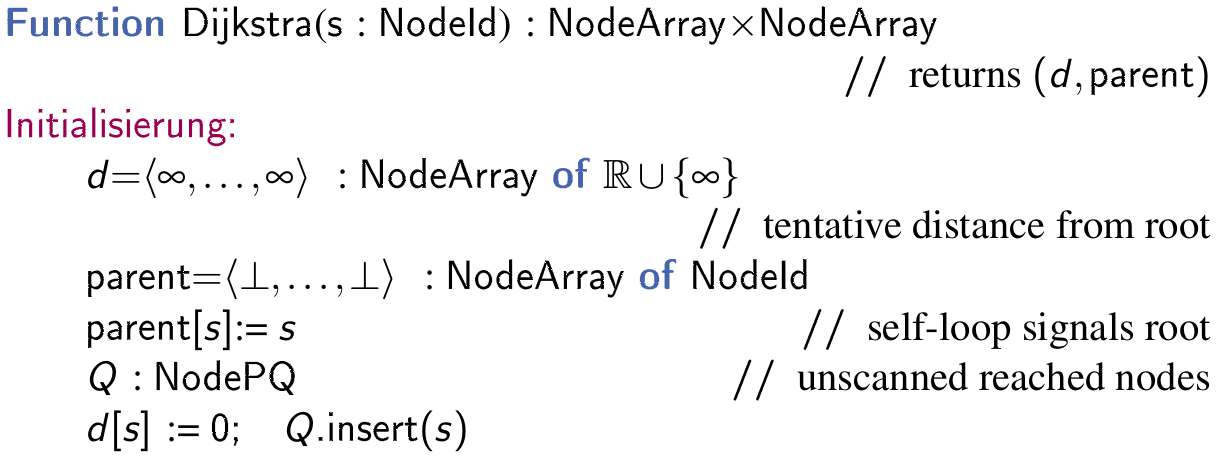
\includegraphics[width=\textwidth]{dijkstra_init}
\end{frame}

\begin{frame}{Dijkstra}
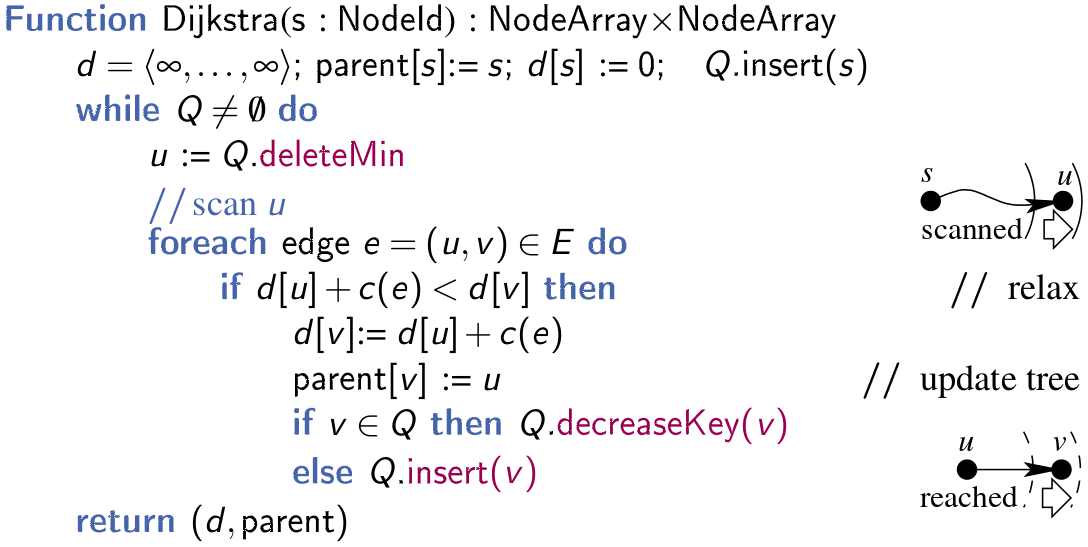
\includegraphics[width=\textwidth]{dijkstra_algo}
\end{frame}

\begin{frame}{Dijkstra Variante}
Beschreibe einen Algorithmus, der in einem Graphen mit Kantengewichten den kürzesten Pfad mit den wenigsten Kanten ausgibt.
\end{frame}

\begin{frame}{Wolf-Ziege-Kohlkopf}
\begin{itemize}
\item Zwei Seiten $A, B$ eines Flusses
\item Ein Fährmann will einen Wolf $W$, eine Ziege $Z$ und einen Kohlkopf $K$ von Seite $A$ auf Seite $B$ befördern
\item In sein Boot passen immer nur er und ein Tier
\item Lässt man Wolf und Ziege alleine, frisst der Wolf die Ziege
\item Lässt man Ziege und Kohlkopf alleine, frisst die Ziege den Kohlkopf
\item Es darf weder die Ziege noch der Kohlkopf gefressen werden
\end{itemize}

Modelliere das Wolf-Ziege-Kohlkopfproblem mit einem Graphen.
\end{frame}

\begin{frame}{Dominosteine}
Gegeben folgende Dominosteine:

\only<1>{1/4}\only<2>{{\color{red}1/6}}, 1/2, 1/5, 1/3, 4/6, 4/2, 4/5, 6/2, 2/5, 5/3

\vspace{1em}
\only<1>{
Es dürfen nur gleiche Zahlen aneinandergelegt werden.
Der Winkel und Abstand aneinanderliegender Steine soll vernachlässigt werden.
Ist es möglich, alle Steine in einen Kreis zu legen?}

\only<2>{
Ändere 1/4 zu 1/6.
Ist es immernoch möglich, alle Steine in einen Kreis zu legen?
Ist es durch entfernen eines Steins möglich, alle übrigen Steine in einen Kreis zu legen?}
\end{frame}

\begin{frame}{Dominosteine}
Was muss im Allgemeinen für eine Menge von Dominosteinen gelten, damit sich aus ihr ein Kreis legen lässt?
\end{frame}

\begin{frame}
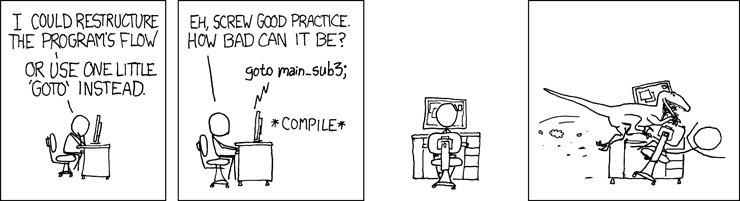
\includegraphics[width=\textwidth]{goto}
\end{frame}

\end{document}
